\subsection{Leader/Follower Design Pattern}
Many systems that process multiple events concurrently need a method to handle 
these events. One common technique is through multi-threading. The 
Leader/Follower pattern, as described in \cite{GangOf4}, is designed for use in
such a system, to provide the means to develop a high performance multi-threaded
system. 

\begin{figure}
  \begin{center}
  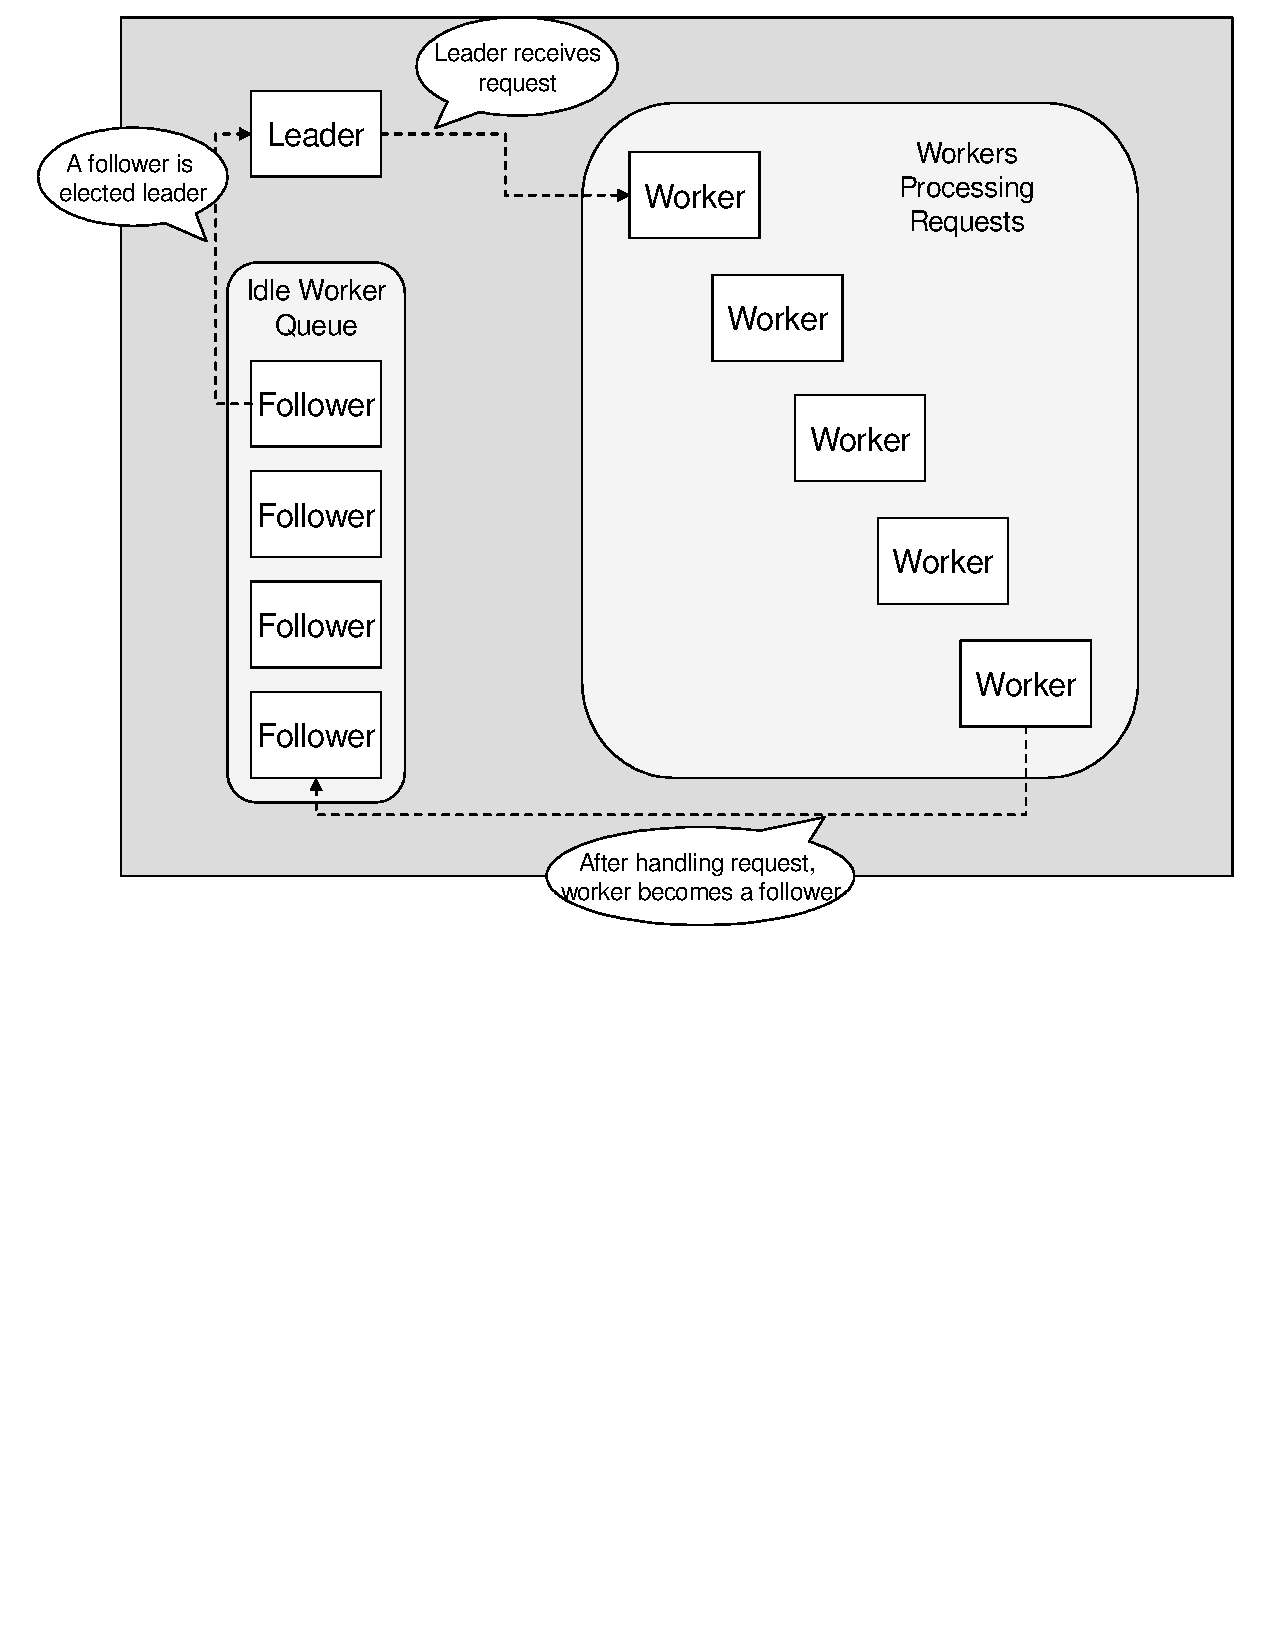
\includegraphics[width=0.9\textwidth]{./images/leaderFollower}
  \caption{Leader/Follower Control Flow}
  \label{fig:leaderFollower}
  \end{center}
\end{figure}

There are three main types of collaborators in the leader-follower pattern: the
leader, follower, and worker as shown in Figure~\ref{fig:leaderFollower}. These
three types of actors are threads in the system. The thread acting as a leader 
waits for an event to occur. The other threads are acting as followers and thus
are waiting to become a leader to handle an event. Once the leader detects an 
event, it designates one of the followers to become the new leader, and then 
becomes a worker thread. In this state, the thread handles the event.  Multiple
worker threads can run concurrently, each handling an event. After the 
processing thread completes its task, it joins the followers thread queue and
again waits its turn to become the leader thread.

\subsubsection{Apache Multitasking Architectures}
Apache has a few multitasking architectures that are supported for different 
operating systems such as Unix and Windows. For Coursebook, the architecture 
that we felt fit best was the Worker Multiprocessing Model, as described in 
\cite{Apache} and shown in Figure~\ref{fig:apache}. This multiprocessing model 
(MPM) uses a combination of multiprocessing and multi-threading techniques. The 
Working MPM is based on the default architecture for Unix systems, the 
pre-forking architecture. This architecture follows the Leader/Follower design
pattern. The main component of the pre-forking architecture is a pool of 
processes. The process pool is created when the master server starts up. These
processes are created before any requests are made; they are ``pre-forked'', 
hence the name of the architecture. Each of these processes is a child server
process. At any given point these child servers can be a leader, follower, or
worker process. A child server starts as a follower, where it sits in a queue
waiting to become a leader. When it is appointed to become a leader, it receives
a connection request and becomes a worker process. In this state, the child
server processes HTTP requests. After completing its requests, the child server
returns to the follower queue and waits its turn to become leader again. The
master server of this architecture controls the number of followers in a queue,
and thus the number of idle processes, to be within a given range to minimize
the server's response time to requests. 

Though the Worker MPM is based upon the pre-forking architecture, it has an
important difference that makes it suitable for Coursebook. The Worker MPM
introduces a multi-threading technique to the multiprocessing technique of the
pre-forking architecture. The Worker MPM utilizes a two-tiered Leader/Follower
design pattern. The first Leader/Follower design is emulated in the child server
processes, as discussed above. The second Leader/Follower design is emulated
within each of these child server processes. A child server process contains two
queues: a job queue and a thread queue. As requests are accepted, they are added
to the job queue. The thread queue contains any follower threads that are idle.
Just as in the Leader/Follower design pattern, a leader thread waits until a
request is received and promotes another follower to be leader before it handles
an incoming request. After completing the request, the leader returns to the
thread queue and becomes a follower again. A child server process will only
accept requests if there are followers in the thread queue, meaning that at
least one idle thread is available to handle a request. 

\begin{figure}
\begin{center}
  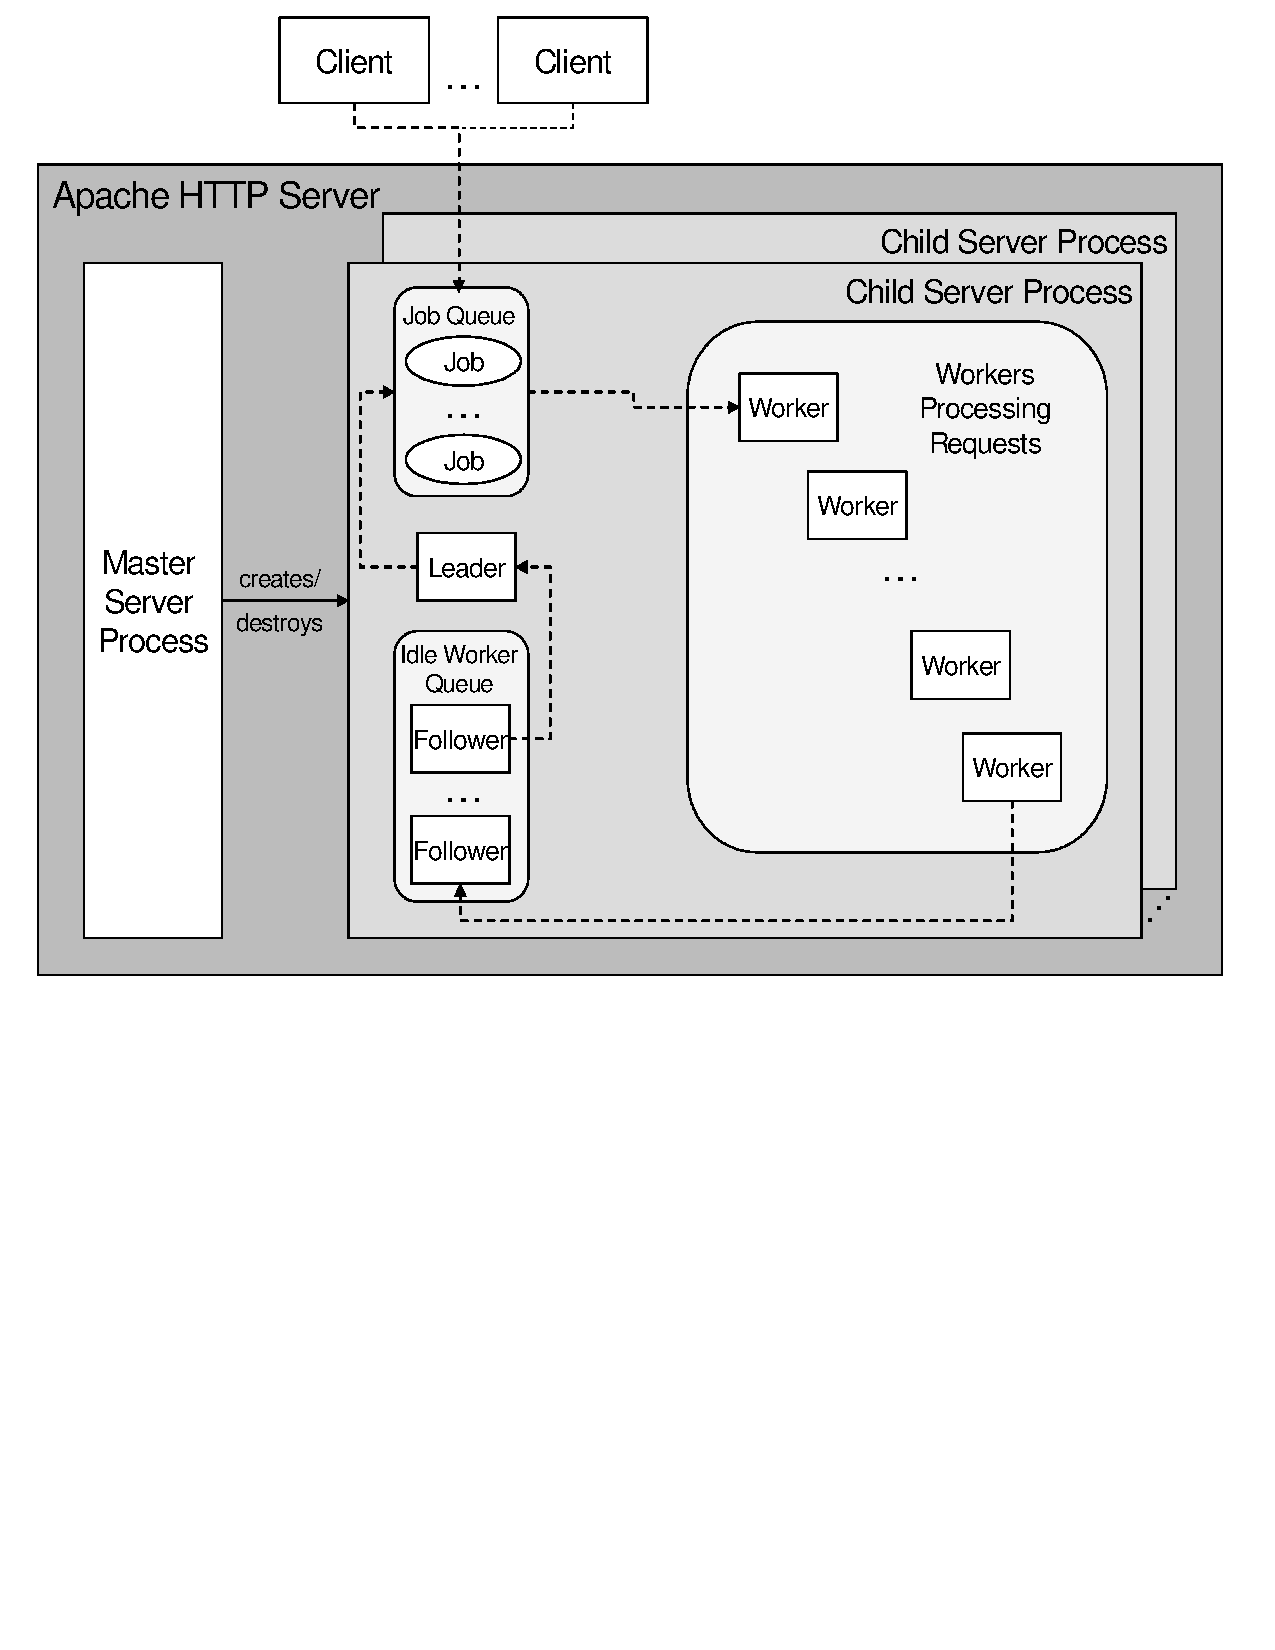
\includegraphics[width=0.9\textwidth]{./images/apacheLeaderFollower}
  \caption{Apache's Use of Leader/Follower}
  \label{fig:apache}
\end{center}
\end{figure}

This two-tiered Leader/Follower design pattern in the Worker MPM combines the
advantages of multiprocessing techniques with those of multi-threading
techniques. Multiprocessing provides stability and fault tolerance
\cite{Apache}, since a failed process does not affect other running processes. A
system that encounters a failed process can handle the failure through the other
running processes. On the other hand, a failed process in a multi-threading
environment affects all of the threads that that parent process had created.
Despite this disadvantage, multi-threading can be advantageous in terms of memory
and performance \cite{Apache}. Threads are more lightweight, thus inferring less
performance overhead in creating threads, and require less memory than
processes during runtime. Therefore, designing an architecture that utilizes
both these techniques can provide a design that is more stable, fault tolerant,
with higher performance and minimal memory usage compared to an architecture
using just one of these techniques \cite{Apache}.
